\chapter{Array Design}
\section{Physical Design}
The 22 week fetal array is designed to provide good surface area coverage and close physical fit on a range of body
types at 22 weeks of pregnancy.  It consists of a rigid posterior panel that attaches directly to the patient table and
a group of anterior and lateral panels that can be freely positioned on the patient. The two lateral panels are attached
to the anterior panel with hinges to provide a degree of freedom. The patient facing surfaces of these panels are
modeled after segmented images of a 22 weeks pregnant volunteer. The precise geometry of the hinged panel assembly was
arrived at through iterative fit tests on pregnant volunteers.
 
The coil formers and housings were designed in Rhinoceros (Robert McNeel \& Associates, WA, USA) and printed in
poly carbonate on a Fortus 400mc 3D printer (Stratasys, Ltd., MN, USA).

\begin{figure}
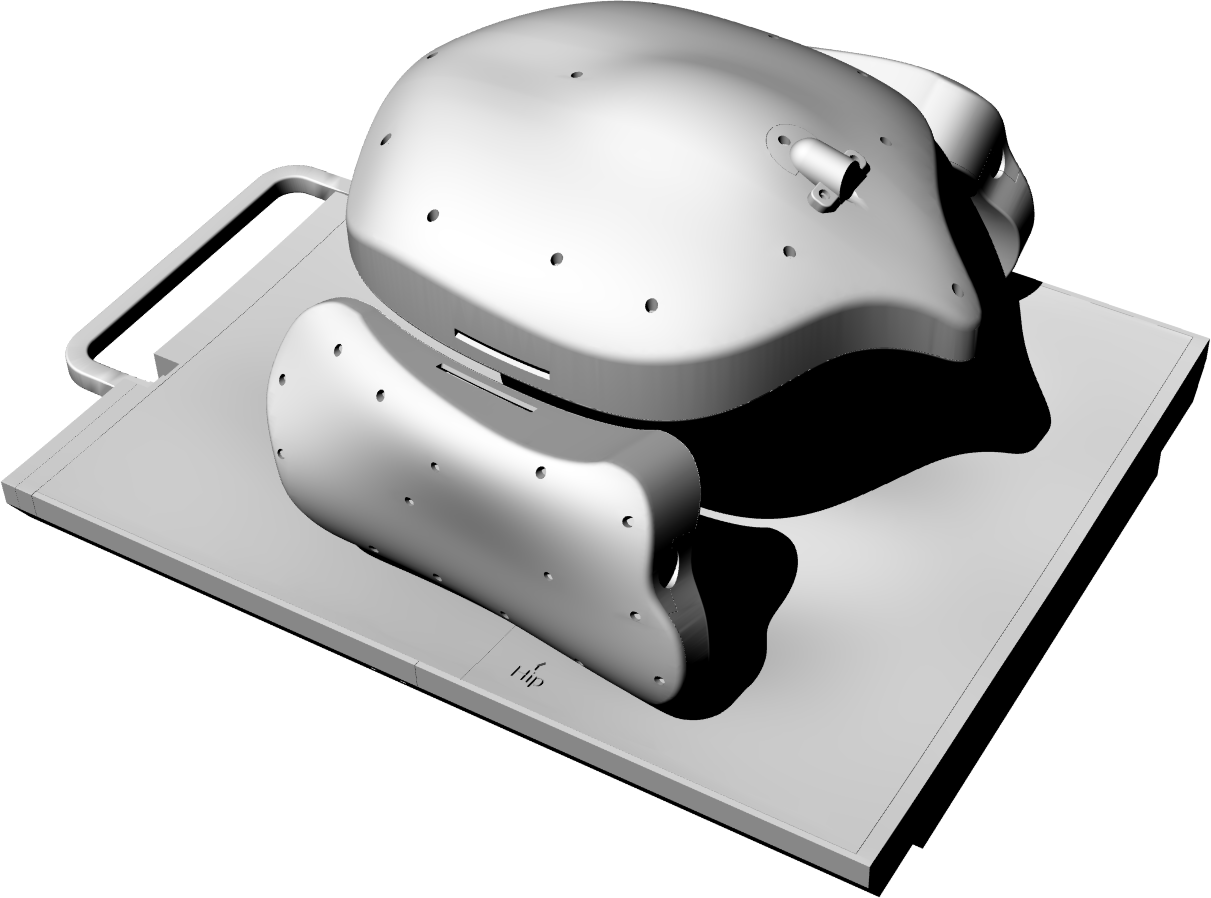
\includegraphics[width=6in]{figures/cad_rendering.png}
\caption{Computer rendering of array panels and housings.}
\label{fig:cad_rendering}
\end{figure}

\section{Array Construction}
The array consists of four distinct groups of coil elements. The posterior panel contains 24 loops, each with a diameter
of approximately 9cm. The anterior panel contains 20 loops, with a median loop diameter of 8cm and with several outliers
in the non-hexagonally tiled area. The two anterior panels contain 10 7cm loops each. The loops in each panel are for
the most part arranged in a hexagonal tiling pattern that allows each loop to be critically overlapped with all of its
neighbors,  thus minimizing inductive coupling between neighboring loops \cite{Roemer94}. The loop layout is shown in
detail in \ref{fig:loop_snr_contributions}.

Individual loops were constructed from 16 gauge tin plated copper wire, with bridges bent into the wires to allow them
to cross each other without touching. A schematic of the loop circuitry is shown in \ref{fig:loop_schematic}. Chapter 4
contains a detailed explanation of the function of the loop circuit.

The finished coil is shown in figure \ref{fig:assembled_view} posed on the pregnant abdomen phantom used extensively
in testing. A view of the internal construction and wiring is shown in figure \ref{fig:internals_composite}.

\begin{figure}
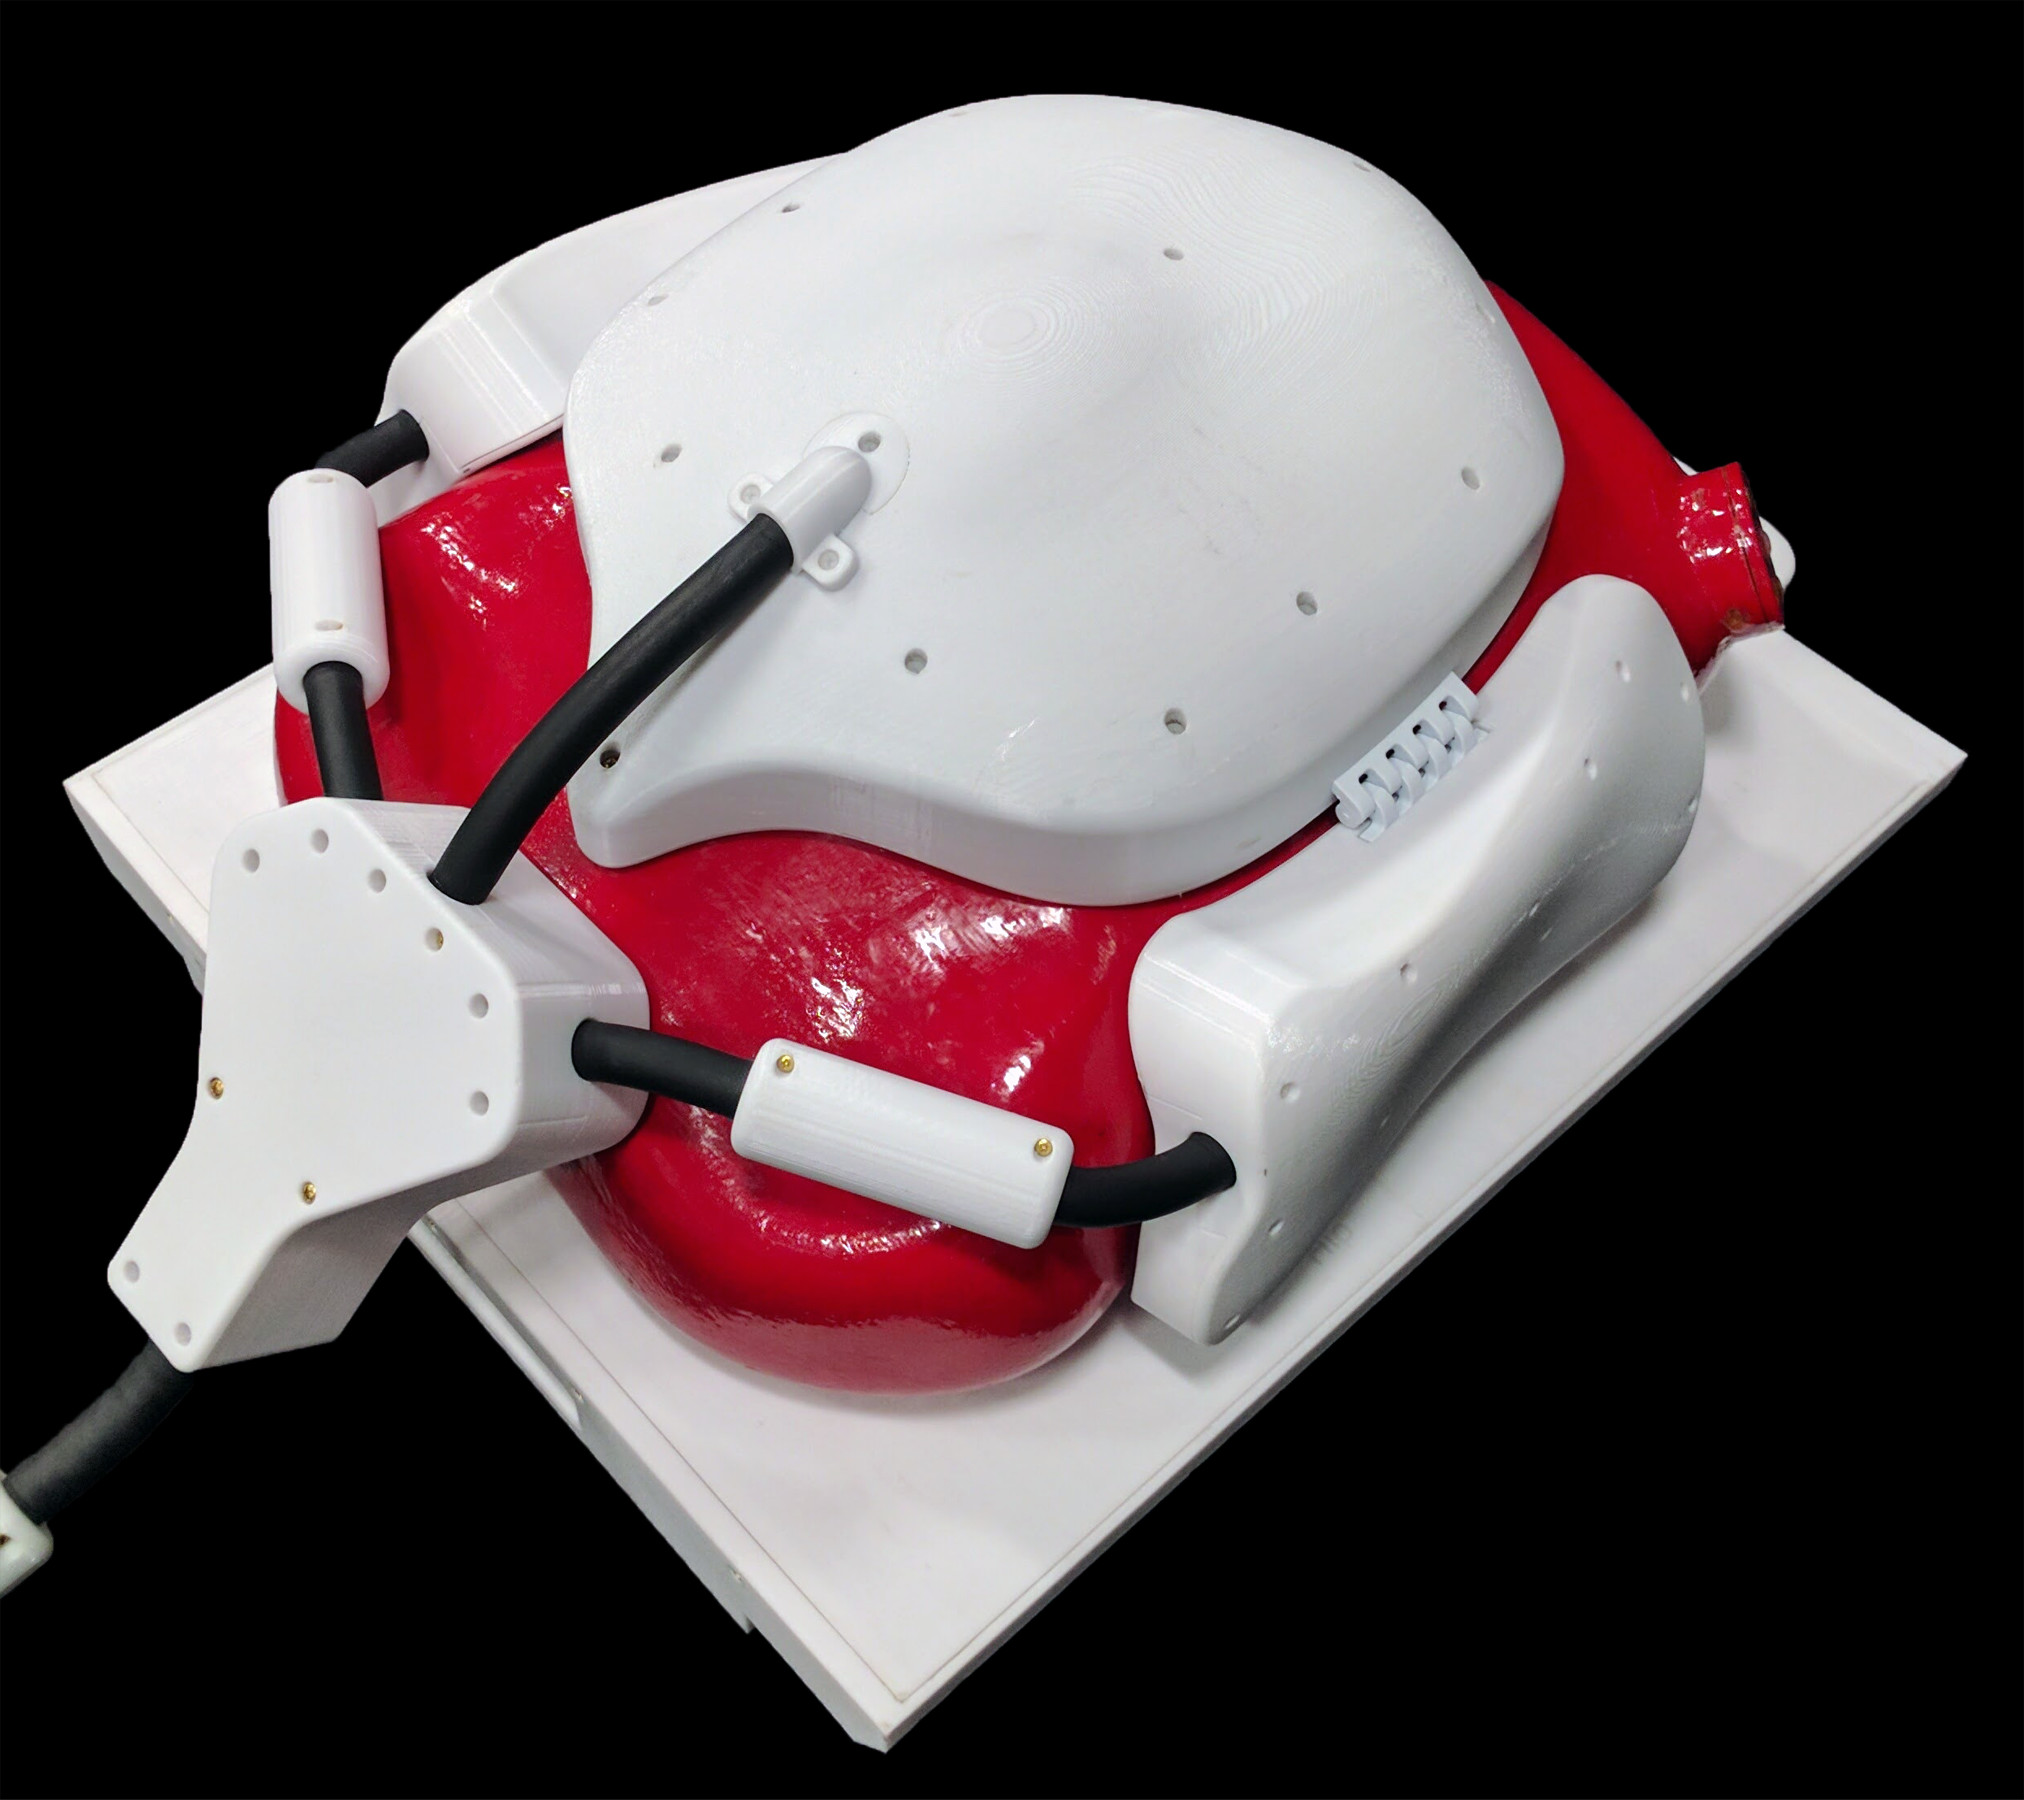
\includegraphics[width=6in]{figures/assembled_view.jpg}
\caption{Finished coil, posed on 22 week pregnant abdomen phantom.}
\label{fig:assembled_view}
\end{figure}

\begin{figure}
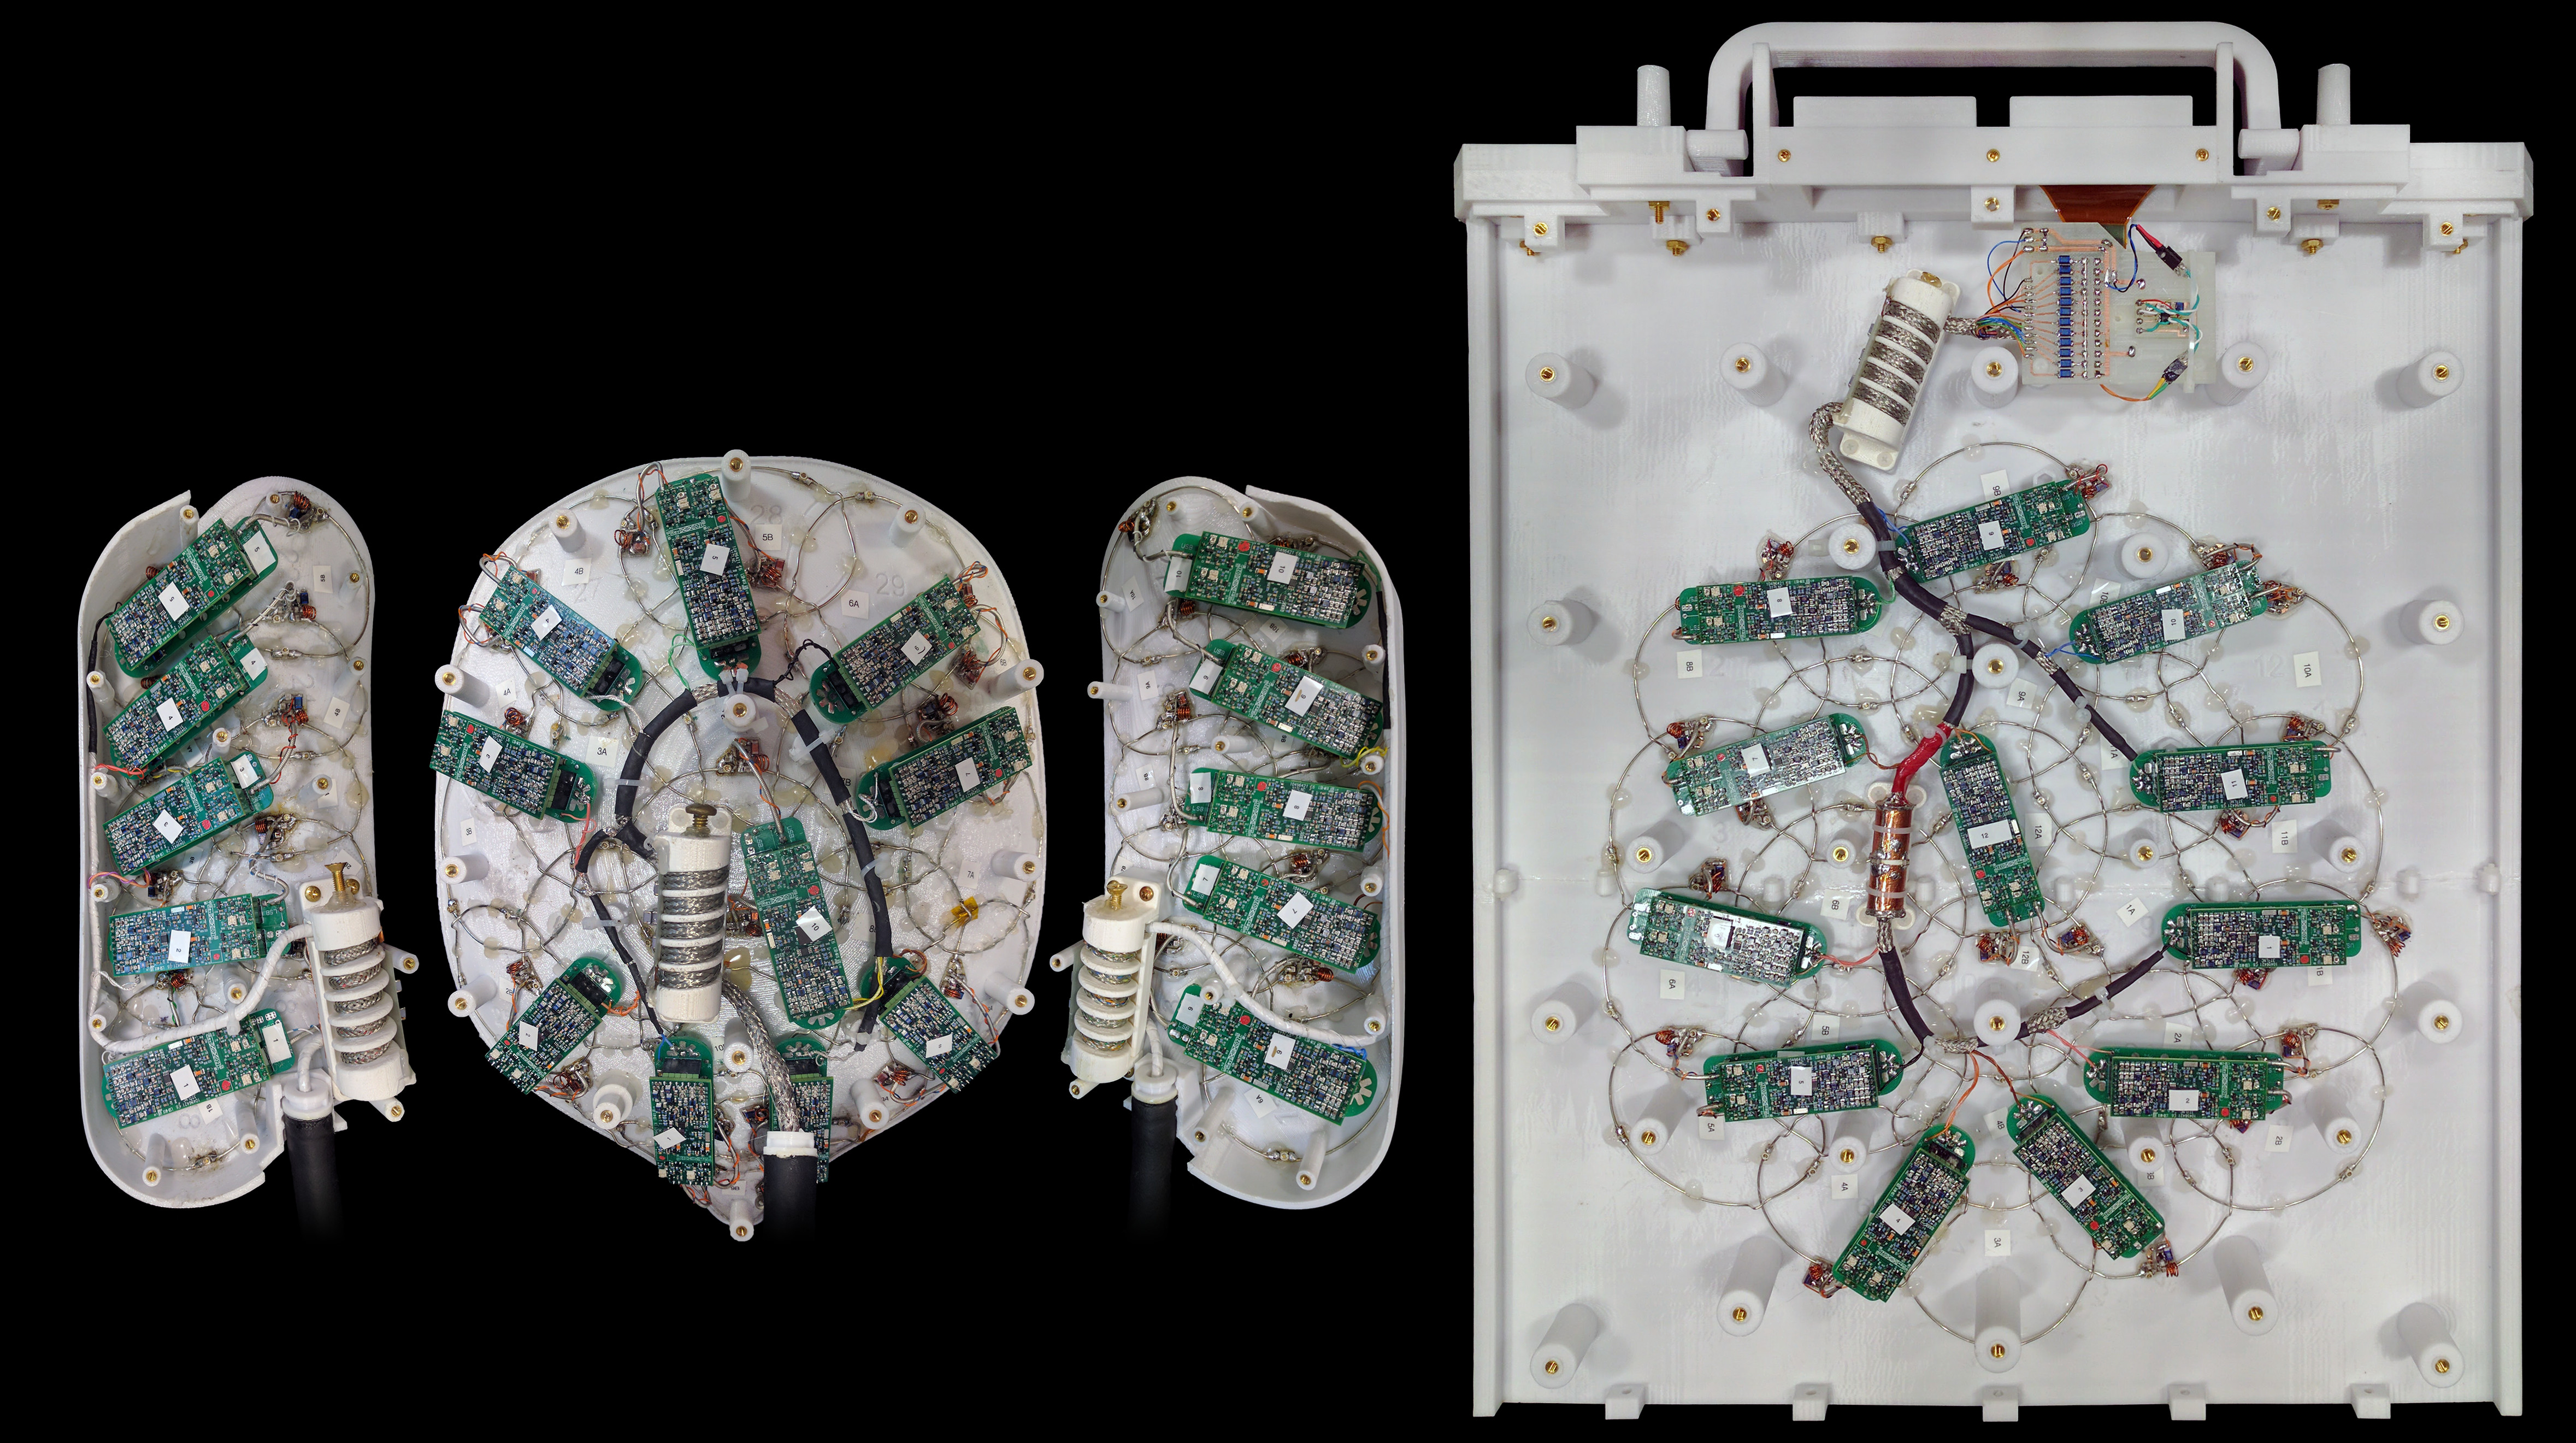
\includegraphics[width=6in]{figures/internals_composite.jpg}
\caption{View of internal array construction and wiring.}
\label{fig:internals_composite}
\end{figure}

\section{Cable Traps}
Precautions must be taken to prevent large currents from developing on internal and external wiring during the RF
transmit phase. Such uncontrolled currents could pose a fire/safety hazard, and at the very least would interfere with
the sequence being run. Common mode chokes spaced every 20cm on all internal and external prevent the induced currents
from growing too large. Due to the high magnetic field the array operates in, ferrite chokes are not an option. Instead,
tuned resonant traps are constructed. Two types of traps were used in this array.

\subsection{Helical Traps}
The operation of the resonant helical traps visible in fig. \ref{fig:internals_composite} is easy to understand.  The
jacketed wire bundle is wound around a helical former, forming an air core inductor. High voltage capacitors are then
connected across the turns of the inductor, forming a parallel LC tank. At resonance, the trap presents a high impedance
to common mode currents flowing in the jacket.  This kind of trap can hold off hundreds of volts, and has a high Q. It
is used as the first cable trap inside each array panel, and inside the table plug.

\subsection{Bazooka Trap}

The bazooka trap can be thought of as a physically short bazooka balun that has been electrically lengthened to
$\frac{\lambda}{4}$ by shunting the open end with a capacitor. A cylindrical plastic spacer is printed in two halves.
The outside surface of each half is covered in copper tape, with a gap left in the middle. The two halves are placed
around the wire bundle and soldered together, and each end of the balun is soldered to the braided wire jacket. The gap
in the copper tape is bridged with nonmagnetic capacitors selected such that the structure resonates at the desired
frequency. An additional layer of copper shielding on the balun enclosure stabilizes the capacitance between the two
ends of the balun so that external loading does not affect its resonant frequency.  This kind of trap is more compact
and consumes less wire length than the helical trap, but cannot hold off as much voltage and has a lower Q. It is
placed periodically on long runs of external wiring.

\begin{figure}
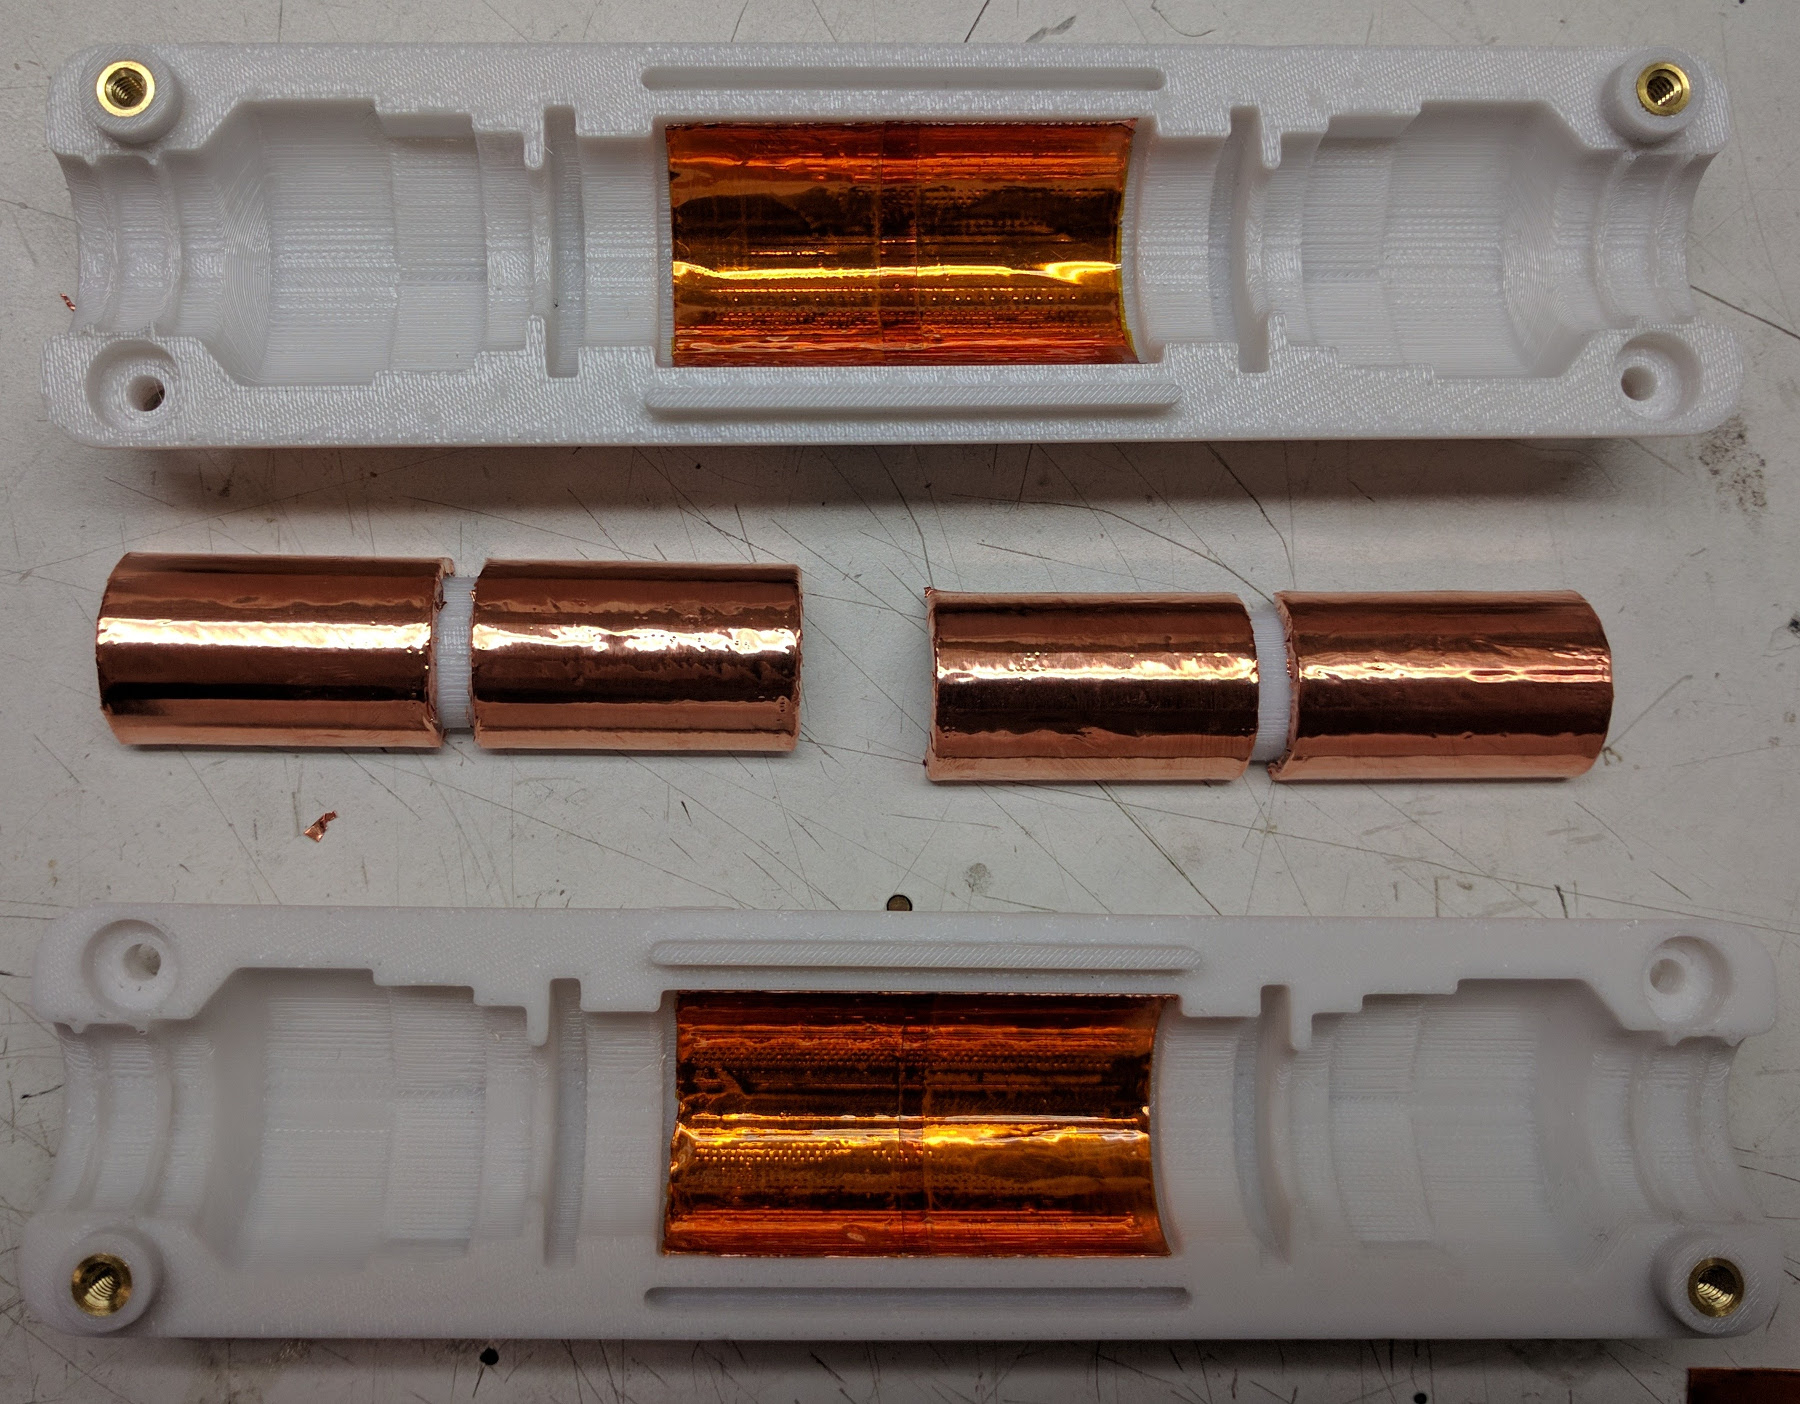
\includegraphics[width=6in]{figures/bazooka_parts.jpg}
\caption{Bazooka Balun before assembly.}
\label{fig:bazooka_parts}
\end{figure}

\begin{figure}
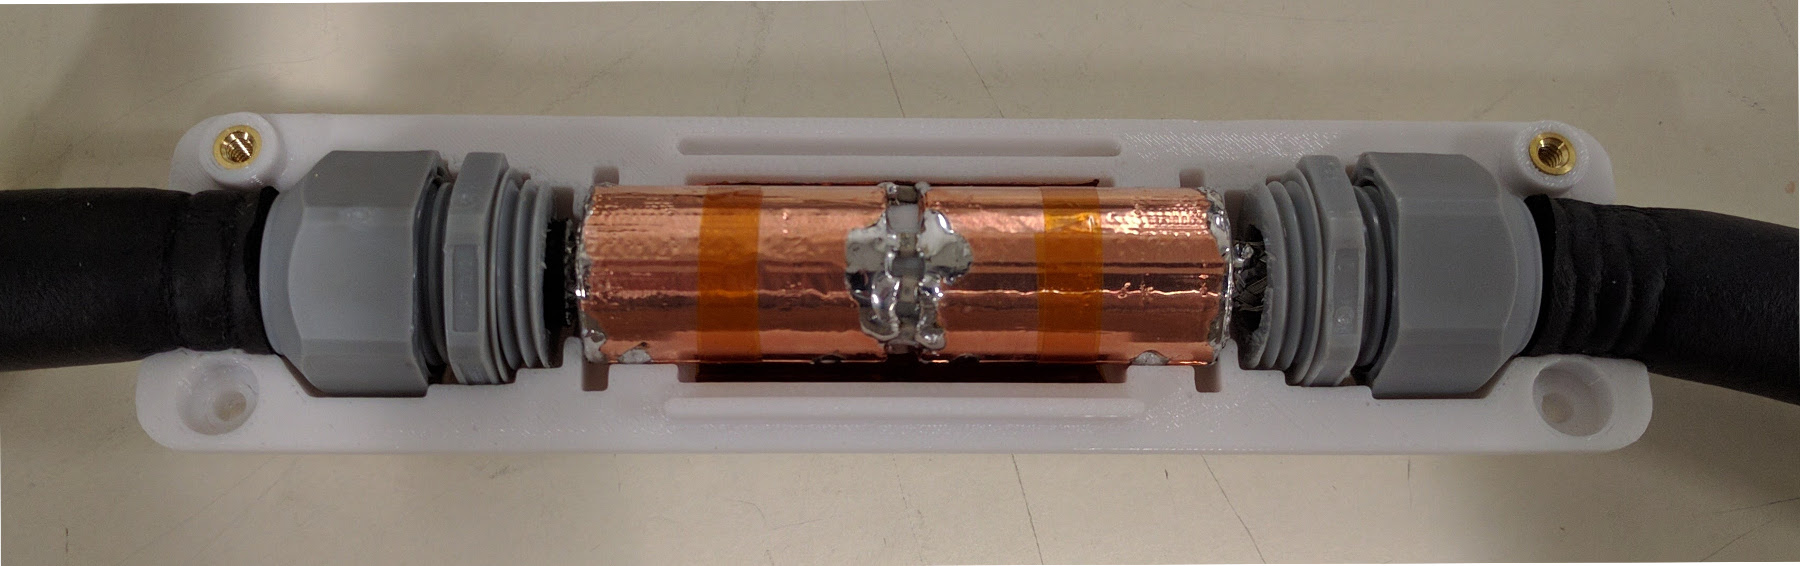
\includegraphics[width=6in]{figures/bazooka_assembled.jpg}
\caption{Completed bazooka balun with open enclosure.}
\label{fig:bazooka_assembled}
\end{figure}

\subsection{Trap Tuning}
Both of the cable trap types described are narrow band, and must be properly tuned to function. This is accomplished
through the use of a network analyzer and two current injection probes (fig. \ref{fig:bazooka_under_test}). Under the
right measurement conditions, a prominent dip (~$20dB$) in $|S_{12}|$ around the resonance frequency can be observed.

\begin{figure}
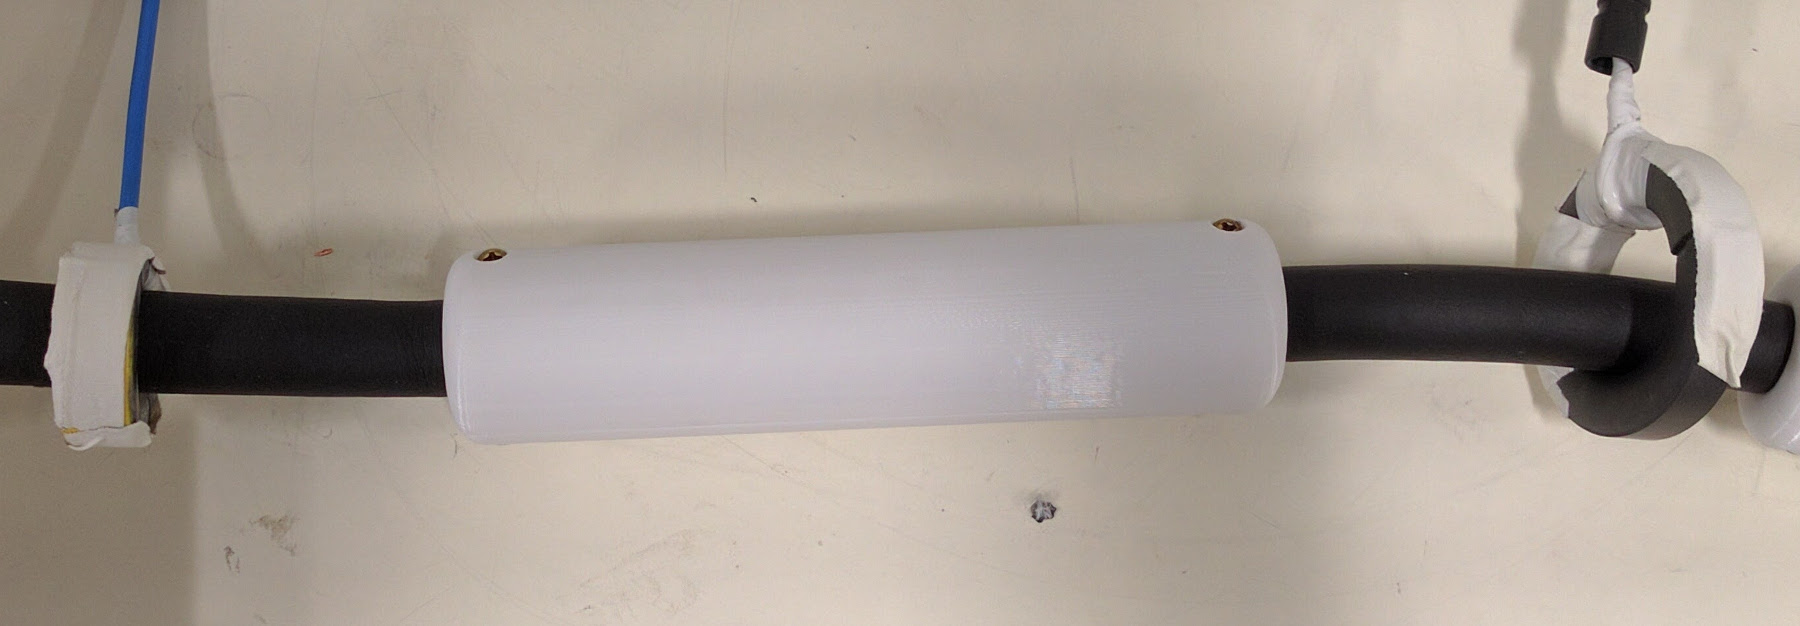
\includegraphics[width=6in]{figures/bazooka_under_test.jpg}
\caption{Cable trap with current injection probes.}
\label{fig:bazooka_under_test}
\end{figure}
